\section{Inversive geometry: keeping the operator inside the space of circles}\label{sec:inv}
The operator $R_i$ turns a circle into a hyperbola, so it leaves the family of circles. Inversive (Möbius) geometry treats circles and lines as one kind of object, which suggests a better question: is there a version of the ``hidden $\leftrightarrow$ visible'' swap that stays inside the space of circles?

\subsection{The space of circles}
A generalized circle is $a(x^2+y^2)+bx+cy+d=0$, up to scale, i.e.\ a point $[a:b:c:d]\in\mathbb{P}^3$. Lines are the case $a=0$, and $\infty:=[0:0:0:1]$ is the point at infinity. Put
\[ Q(C)=b^2+c^2-4ad,\qquad \langle C_1,C_2\rangle=b_1b_2+c_1c_2-2(a_1d_2+a_2d_1). \]
Since $Q=b^2+c^2+(a-d)^2-(a+d)^2$, the form has signature $(3,1)$. For $a\neq0$ the centre is $(-b/2a,-c/2a)$ and $Q=4a^2r^2$. So $Q>0$ is a real circle (every real line has $Q=b^2+c^2>0$), $Q=0$ a point circle, and $Q<0$ an imaginary circle such as $x^2+y^2+1=0$ ($Q=-4$). A point $p$ is the point circle $P(p)=[1:-2x:-2y:|p|^2]$, and
\[ \langle P(p),C\rangle=-2\,C(p), \]
so \emph{incidence is orthogonality}: $p\in C\iff P(p)\perp C$. The points of the inversive plane $\R^2\cup\{\infty\}\cong S^2$ form the null quadric $\{Q=0\}$. For two real circles with radii $r_1,r_2$ and centre distance $\delta$, $\langle C_1,C_2\rangle/\sqrt{Q_1Q_2}=(r_1^2+r_2^2-\delta^2)/(2r_1r_2)=\cos\theta$, where $\theta$ is the intersection angle. For a circle and a line, the same ratio is $\pm\delta/r$, with $\delta$ the distance from the centre to the line. Hence:

\begin{proposition}\label{prop:inv}
For real circles or lines $C_1,C_2$, let $I=\langle C_1,C_2\rangle^2/(Q_1Q_2)$. Then $I<1$ means two real intersection points (at angle $\theta$, $I=\cos^2\theta$), $I=1$ means tangency, and $I>1$ means a conjugate pair of intersection points. For $C_0:x^2+y^2=r^2$ and $L_c:y=c$ (with $d=(1,0)$, $n=(0,1)$), $I=c^2/r^2$.
\end{proposition}
\noindent(Checked on 3000 random circle pairs and 3000 random circle–line pairs: no mismatches, and $|I-\cos^2\theta|<2\cdot10^{-14}$.)

\subsection{The Möbius group}
Inversion in a real circle $C$ acts on $\R^{3,1}$ as the reflection $X\mapsto X-2\frac{\langle X,C\rangle}{Q(C)}C$ (checked numerically to $10^{-12}$). Inversions generate the Möbius group, so it acts \emph{linearly} on circles preserving $Q$: $\mathrm{M\ddot ob}\cong PO(3,1)$, whose orientation-preserving part is $PSO^+(3,1)\cong PSL(2,\C)$. Complexifying gives $PO(4,\C)$, acting on complex circles $\mathbb{P}^3(\C)$ and on the complex null quadric $\{Q=0\}\cong\mathbb{P}^1\times\mathbb{P}^1$, with coordinates $z=x+iy$, $w=x-iy$ on the finite part $\C^2$. The identity component is $PSO(4,\C)\cong PSL(2,\C)\times PSL(2,\C)$, acting by $(z,w)\mapsto(g z,h w)$. The real Möbius plane is the fixed set of the real structure $\sigma_0:(x,y)\mapsto(\bar x,\bar y)$, i.e.\ $w=\bar z$. The two rulings $z=\mathrm{const}$ and $w=\mathrm{const}$ of the quadric are the isotropic lines of \S\ref{sec:iso}.

\subsection{Point pairs as 2-planes}
A pair of points $\{P_1,P_2\}$ (a $0$-sphere) is a 2-plane $U=\mathrm{span}(P_1,P_2)\subset\R^{3,1}$, a line in $\mathbb{P}^3$ meeting the quadric in $P_1,P_2$. Two circles $C_1,C_2$ meet in the null points of $U=V^\perp$, where $V=\mathrm{span}(C_1,C_2)$ is the \emph{pencil} (coaxal system) they span. Because the total signature is $(3,1)$, a real 2-plane is of exactly one of three types:
\begin{center}\begin{tabular}{llll}
signature of $U$ & null points of $U$ & $V=U^\perp$ & $\det\mathrm{Gram}(C_1,C_2)=Q_1Q_2-\langle C_1,C_2\rangle^2$\\\hline
$(1,1)$ & real pair & $(2,0)$: elliptic pencil & $>0$ \ ($I<1$)\\
degenerate & double point & parabolic pencil & $=0$\\
$(2,0)$ & conjugate pair $P,\bar P$ & $(1,1)$: hyperbolic pencil & $<0$ \ ($I>1$)
\end{tabular}\end{center}
The signature $(0,2)$ cannot occur. For a conjugate pair, $u=P+\bar P$ and $v=i(P-\bar P)$ span a real plane with $Q|_U=2\langle P,\bar P\rangle(u^2+v^2)$, which must be positive definite. The null points of $V$ itself are the \emph{limiting points} of the pencil. They are real exactly when the intersection pair is imaginary, and vice versa.

\begin{proposition}[Polarity swaps real and imaginary pairs]\label{prop:polar}
The map $U\mapsto U^\perp$ on point pairs is a Möbius-equivariant involution exchanging real pairs and conjugate pairs. For $C_0$ and $L_c$ it sends the intersection pair $C_0\cap L_c=\{(\pm\sqrt{r^2-c^2},\,c)\}$ to the limiting points
\[ \{(0,\;c\pm\sqrt{c^2-r^2})\}, \]
which are mutually inverse in $C_0$ (the product of their $y$-coordinates is $r^2$). For $|c|>r$, with $s=\sqrt{c^2-r^2}$, the hidden pair $(\pm is,c)$ becomes the real pair $(0,c\pm s)$ on the normal through the foot $(0,c)$. Quilez's orange dots $(\pm s,c)$ are the same real pair rotated by $90^\circ$ about the foot.
\end{proposition}
\begin{proof}
$U\mapsto U^\perp$ commutes with every element of $PO(3,1)$, and the table shows it swaps the $(1,1)$ and $(2,0)$ types. With $C_0=[1:0:0:-r^2]$ and $L_c=[0:0:1:-c]$, $Q(\lambda C_0+\mu L_c)=4r^2\lambda^2+4c\lambda\mu+\mu^2$ vanishes at $\mu/\lambda=-2c\pm2\sqrt{c^2-r^2}$. The circle $x^2+y^2+\mu y-r^2-\mu c=0$ then has radius $0$ and centre $(0,-\mu/2)=(0,c\mp\sqrt{c^2-r^2})$.
\end{proof}
\noindent(Numerically, for $r=1$: at $c=1.7$ the null points of $U$ are $(\pm1.37477i,1.7)$ and those of $V$ are $(0,3.07477),(0,0.32523)$. At $c=0.6$ they are $(\pm0.8,0.6)$ and $(0,0.6\pm0.8i)$.)

\begin{figure}[t]\centering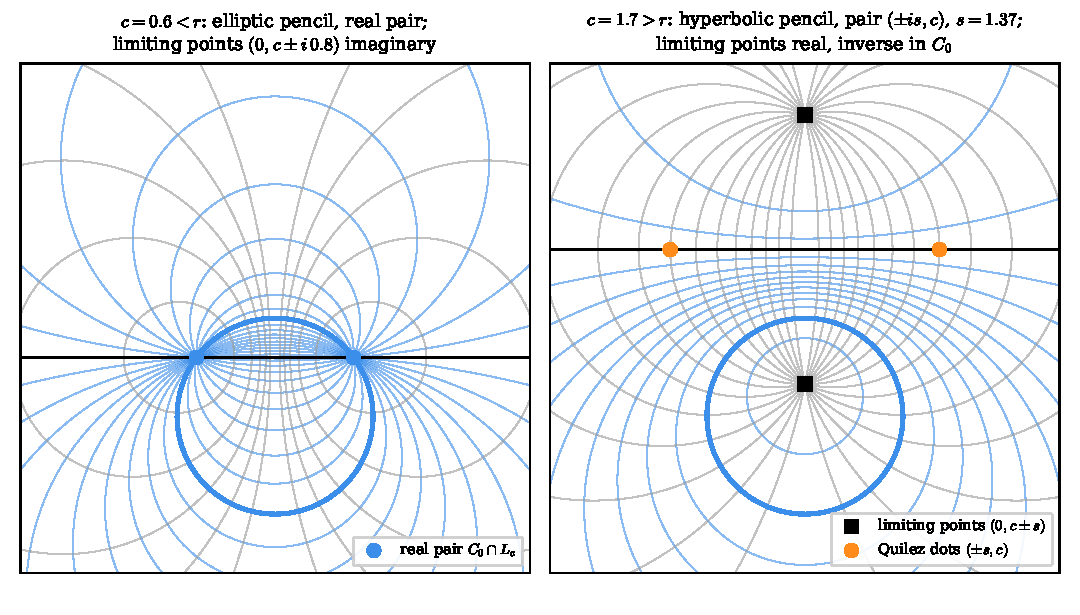
\includegraphics[width=\linewidth]{figs/fig5_pencil.pdf}
\caption{The pencil $V_c=\mathrm{span}(C_0,L_c)$ (thin blue) and its orthogonal pencil $V_c^\perp$ (grey), for $r=1$. Left, $c=0.6$: elliptic pencil through the real pair $C_0\cap L_c$, with imaginary limiting points. Right, $c=1.7$: the pair is $(\pm is,c)$; the pencil is hyperbolic with real limiting points $(0,c\pm s)$ (squares), through which every grey circle passes. Quilez's dots $(\pm s,c)$ (orange) are the limiting points rotated by $90^\circ$ about the foot $(0,c)$.}\label{fig:pencil}\end{figure}

\subsection{Why \texorpdfstring{$R_i$}{R\_i} is not internal, and what replaces it}
Write $M=R_{-1}:(x,y)\mapsto(-x,y)$ for the mirror in the $n$-axis, which is a real Möbius map.

\begin{theorem}\label{thm:inv}
Let $C_0:x^2+y^2=r^2$ and the parallel pencil $\mathcal{P}=\{L_c:y=c\}$.
\begin{enumerate}
\item $R_i$ is not induced by any element of $PO(4,\C)$. It sends the circular points $(1:\pm i:0)$ to the real points $(1:\pm1:0)$, so it sends circles (conics through the circular points) to non-circles; $C_0$ goes to the hyperbola $y^2-x^2=r^2$.
\item The subgroup of $PO(4,\C)$ preserving $C_0$ and $\mathcal{P}$ is the Klein four-group $\{\mathrm{id},\,-\mathrm{id},\,M,\,(x,y)\mapsto(x,-y)\}$. It consists of real maps and contains $R_i^2=M$, but not $R_i$. So no element of the complexified circle group fixing the configuration exchanges real and imaginary point pairs.
\item The exchange is a \emph{change of real structure}. Let $\sigma_1=\sigma_0\circ M:(x,y)\mapsto(-\bar x,\bar y)$. It is an anti-holomorphic involution that preserves the circle family and fixes $C_0$ and every $L_c$, and $\sigma_1=R_i\sigma_0R_i^{-1}$. On each pair $C_0\cap L_c$, $\sigma_0$ fixes both points when $|c|<r$ and swaps them when $|c|>r$, while $\sigma_1$ does the opposite. The $\sigma_1$-real points of $C_0$ are $\{(is,c):c^2-s^2=r^2\}$, the phantom hyperbola.
\item The $\sigma_1$-real circles are $[a:i\beta:c:d]$ with $a,\beta,c,d$ real, on which $Q=-\beta^2+c^2-4ad$ has signature $(2,2)$. So $\sigma_1$ is the real form $PO(2,2)$ of $PO(4,\C)$: the conformal geometry of the \emph{Lorentzian} plane $\{(is,c)\}$ with metric $dc^2-ds^2$, whose ``circles'' are hyperbolas. In that geometry, the phantom of the circle is the Lorentzian circle of the same radius.
\end{enumerate}
\end{theorem}
\begin{proof}
(1) $R_i$ multiplies the top-degree form $x^2+y^2$ into $y^2-x^2$, which does not vanish at $(1:\pm i)$. Equivalently, the induced map on point vectors $[1:-2x:-2y:x^2+y^2]\mapsto[1:-2ix:-2y:y^2-x^2]$ is not linear: the best linear fit on 12 random points leaves residual $2.04$.
(2) Every pencil member passes through $\infty$, and $\infty$ is the only base point of $\mathcal{P}$ (the null points of $\mathcal{P}^\perp$ reduce to $[0:0:0:1]$). So the stabilizer fixes $\infty$ and consists of complex similarities $(z,w)\mapsto(\alpha z+a,\beta w+b)$, or the same composed with $z\leftrightarrow w$. Preserving $zw=r^2$ forces $a=b=0$ and $\alpha\beta=1$. Mapping the lines $z-w=2ic$ to lines of the same form forces $\alpha=\beta$. Hence $\alpha=\pm1$ (solved symbolically).
(3) For $\sigma_1=R_i\sigma_0R_i^{-1}$: $(x,y)\mapsto(-ix,y)\mapsto(i\bar x,\bar y)\mapsto(-\bar x,\bar y)$. $\sigma_1$ preserves circles because $\sigma_0$ and $M$ do. On $C_0\cap L_c=\{(\pm\xi,c)\}$, $\sigma_0$ fixes each point iff $\xi\in\R$, and $\sigma_1(\xi,c)=(-\bar\xi,c)$ fixes each point iff $\xi\in i\R$.
(4) Points fixed by $\sigma_1$ are $(is,c)$ with $s,c$ real, and $P(is,c)=[1:-2is:-2c:c^2-s^2]$ has the stated form.
\end{proof}

\noindent\textbf{Summary.} Inside the space of circles there are two honest replacements for $t\mapsto it$, and neither is a group element fixing the configuration.
(a) The \emph{polarity} $U\mapsto U^\perp$ is a real, Möbius-equivariant operation on point pairs. It sends the hidden pair of $C_0$ and $L_c$ to the real limiting points of the pencil they span.
(b) Swapping which points count as real is a change of real form, $PO(3,1)\to PO(2,2)$, implemented by $\sigma_1=\sigma_0M$. The two real forms are not conjugate in $PO(4,\C)$, because a conjugating element would carry a real 4-space of signature $(3,1)$ to one of signature $(2,2)$ while scaling $Q$. In this language, $R_i$ is a square root of the Möbius mirror $M$ that lives outside the Möbius group and intertwines the two real structures. The circle and its phantom are one complex circle, seen through the Euclidean and the Lorentzian real structure.
